\section{Rotor do sterowania antenami w płaszczyźnie azymutu i elewacji}

Konstrukcja rotora składa się z dwóch stalowych skrzynek osłaniających silniki. W skrzynkach zostały wykonane otwory na poprowadzenie przewodów do zasilania i sterowania.

Aby uzyskać dużą precyzję i wytrzymały na warunki zewnętrzne system pomimo małych gabarytów, potrzebne było duże przełożenie dla silników. Po doborze przekładni pełen obrót w płaszczyźnie azymutu zajmuje 124 sekundy, a w płaszczyźnie elewacji 64 sekundy. Wolny czas obrotu zwykle w rotorach antenowych nie przeszkadza, ponieważ zwykle nie namierza się szybko poruszających się źródeł sygnału. Podane prędkości są dla zasilania napięciem 12 V. Jest możliwe uzyskanie proporcjonalnie szybszych obrotów dostarczając większe napięcie zasilania (np. łącząc dwa akumulatory równolegle). Użyte silniki tolerują napięcie do 30V.

Śledzenie pozycji rotora odbywa się przy pomocy zestawu czujników: 
\begin{itemize}
 \item enkoderów optycznych przed przekładnią (co znacznie poprawia ich rozdzielczość na pełen obrót, ale wprowadza trochę błędu ze względu na luzy w przekładniach)
 \item zamontowanego do osi z na anteny układu czujników \emph{pololu} zawierającego kompas magnetyczny, żyroskopy i akcelerometry w trzech osiach, który służy do kalibracji układu.
\end{itemize}

Kalibracja układu polega na ustaleniu na podstawie danych z kompasu aktualnej orientacji rotora względem kierunków geograficznych. Wcześniejsze relatywne położenie rotora jest odczytywane z pamięci stałej EEPROM. Podczas kalibracji wykonuje się też pełen obrót w płaszczyźnie azymutu i wykrywa się przy pomocy akcelerometru czy rotor nie stoi pochylony. W przypadku wykrycia pochyłu do zadawanych położeń obliczana jest dodatkowa korekta.

\begin{figure}[!htbp]
 \includegraphics[width=0.8\textwidth]{rotor}
 \centering
 \caption{Konstrukcja rotora zamontowana na statywie}
\end{figure}

Cała stacja waży około 12 kilogramów. Rotor ma miejsce na przykręcane rury do mocowania anten. Przewidujemy nie więcej niż 2 anteny jednocześnie o łącznej wadze do 8 kilogramów.

Niestety tak jak w większości rotorów (poza zaawansowanymi rozwiązaniami), ze względu na kabel można obracać rotorem w wybranym kierunku tylko w ograniczonym zakresie. Maksymalny kąt obrotu zależy od poprowadzenia przewodu zarówno do anteny jak i zasilających w rotorze. Do zasilania daliśmy zapas kabla na około 2 pełne obroty. Pilnowanie aby nie przekroczyć maksymalnego obrotu odbywa się programowo zapamiętując i wczytując względny obrót w pamięci trwałej. 

Rotor bardzo trudno obrócić bez włączonego zasilania ze względu na duże przełożenie w przekładniach. Jest to zamierzone, aby przy trudniejszych warunkach atmoseferycznych (przede wszystkim wietrze) rotor się nie obracał bez kontroli.

Dolna część rotora zawiera silnik obracający część górną w płaszczyźnie azymutu przy pomocy dwóch przekładni - ślimakowej i planetarnej. W tym przypadku tarcza enkodera została zamontowana pomiędzy przekładniami ze względu na brak wyprowadzenia ośki silnika. Dolna skrzynka jest dość obszerna, żeby móc w środku schować układy elektroniczne (sterownik arduino, mostki H, przetwornica napięcia). Ta część zawiera też otwory na przewody do komputera na kabel USB i przewody do zasilania. Dolna część rotora bez układów elektornicznych została przedstawiona na rysunku \ref{rotdol}.

Górna część rotora znajdująca się na rysunku \ref{rotgora} zawiera silnik obracający oś do mocowania anten w płaszczyźnie elewacji. Do skrzynki dochodzą przewody z dolnej części - przewody: zasilający 12V, zasilający 5V, masy, 2 sterujące silnikiem i przewód z danymi enkodera. Wszystko jest umieszczone w jednym kablu 6-żyłowym skręconym, aby był elastyczny i rozciągliwy. 

W przenośnym rozwiązaniu układ SDR znajduje się w dodatkowym pokrowcu (walizce) umieszczonym pod rotorem, gdzie dochodzi do niego przewód radiowy wprost z anteny.

\begin{figure}[!htbp]
 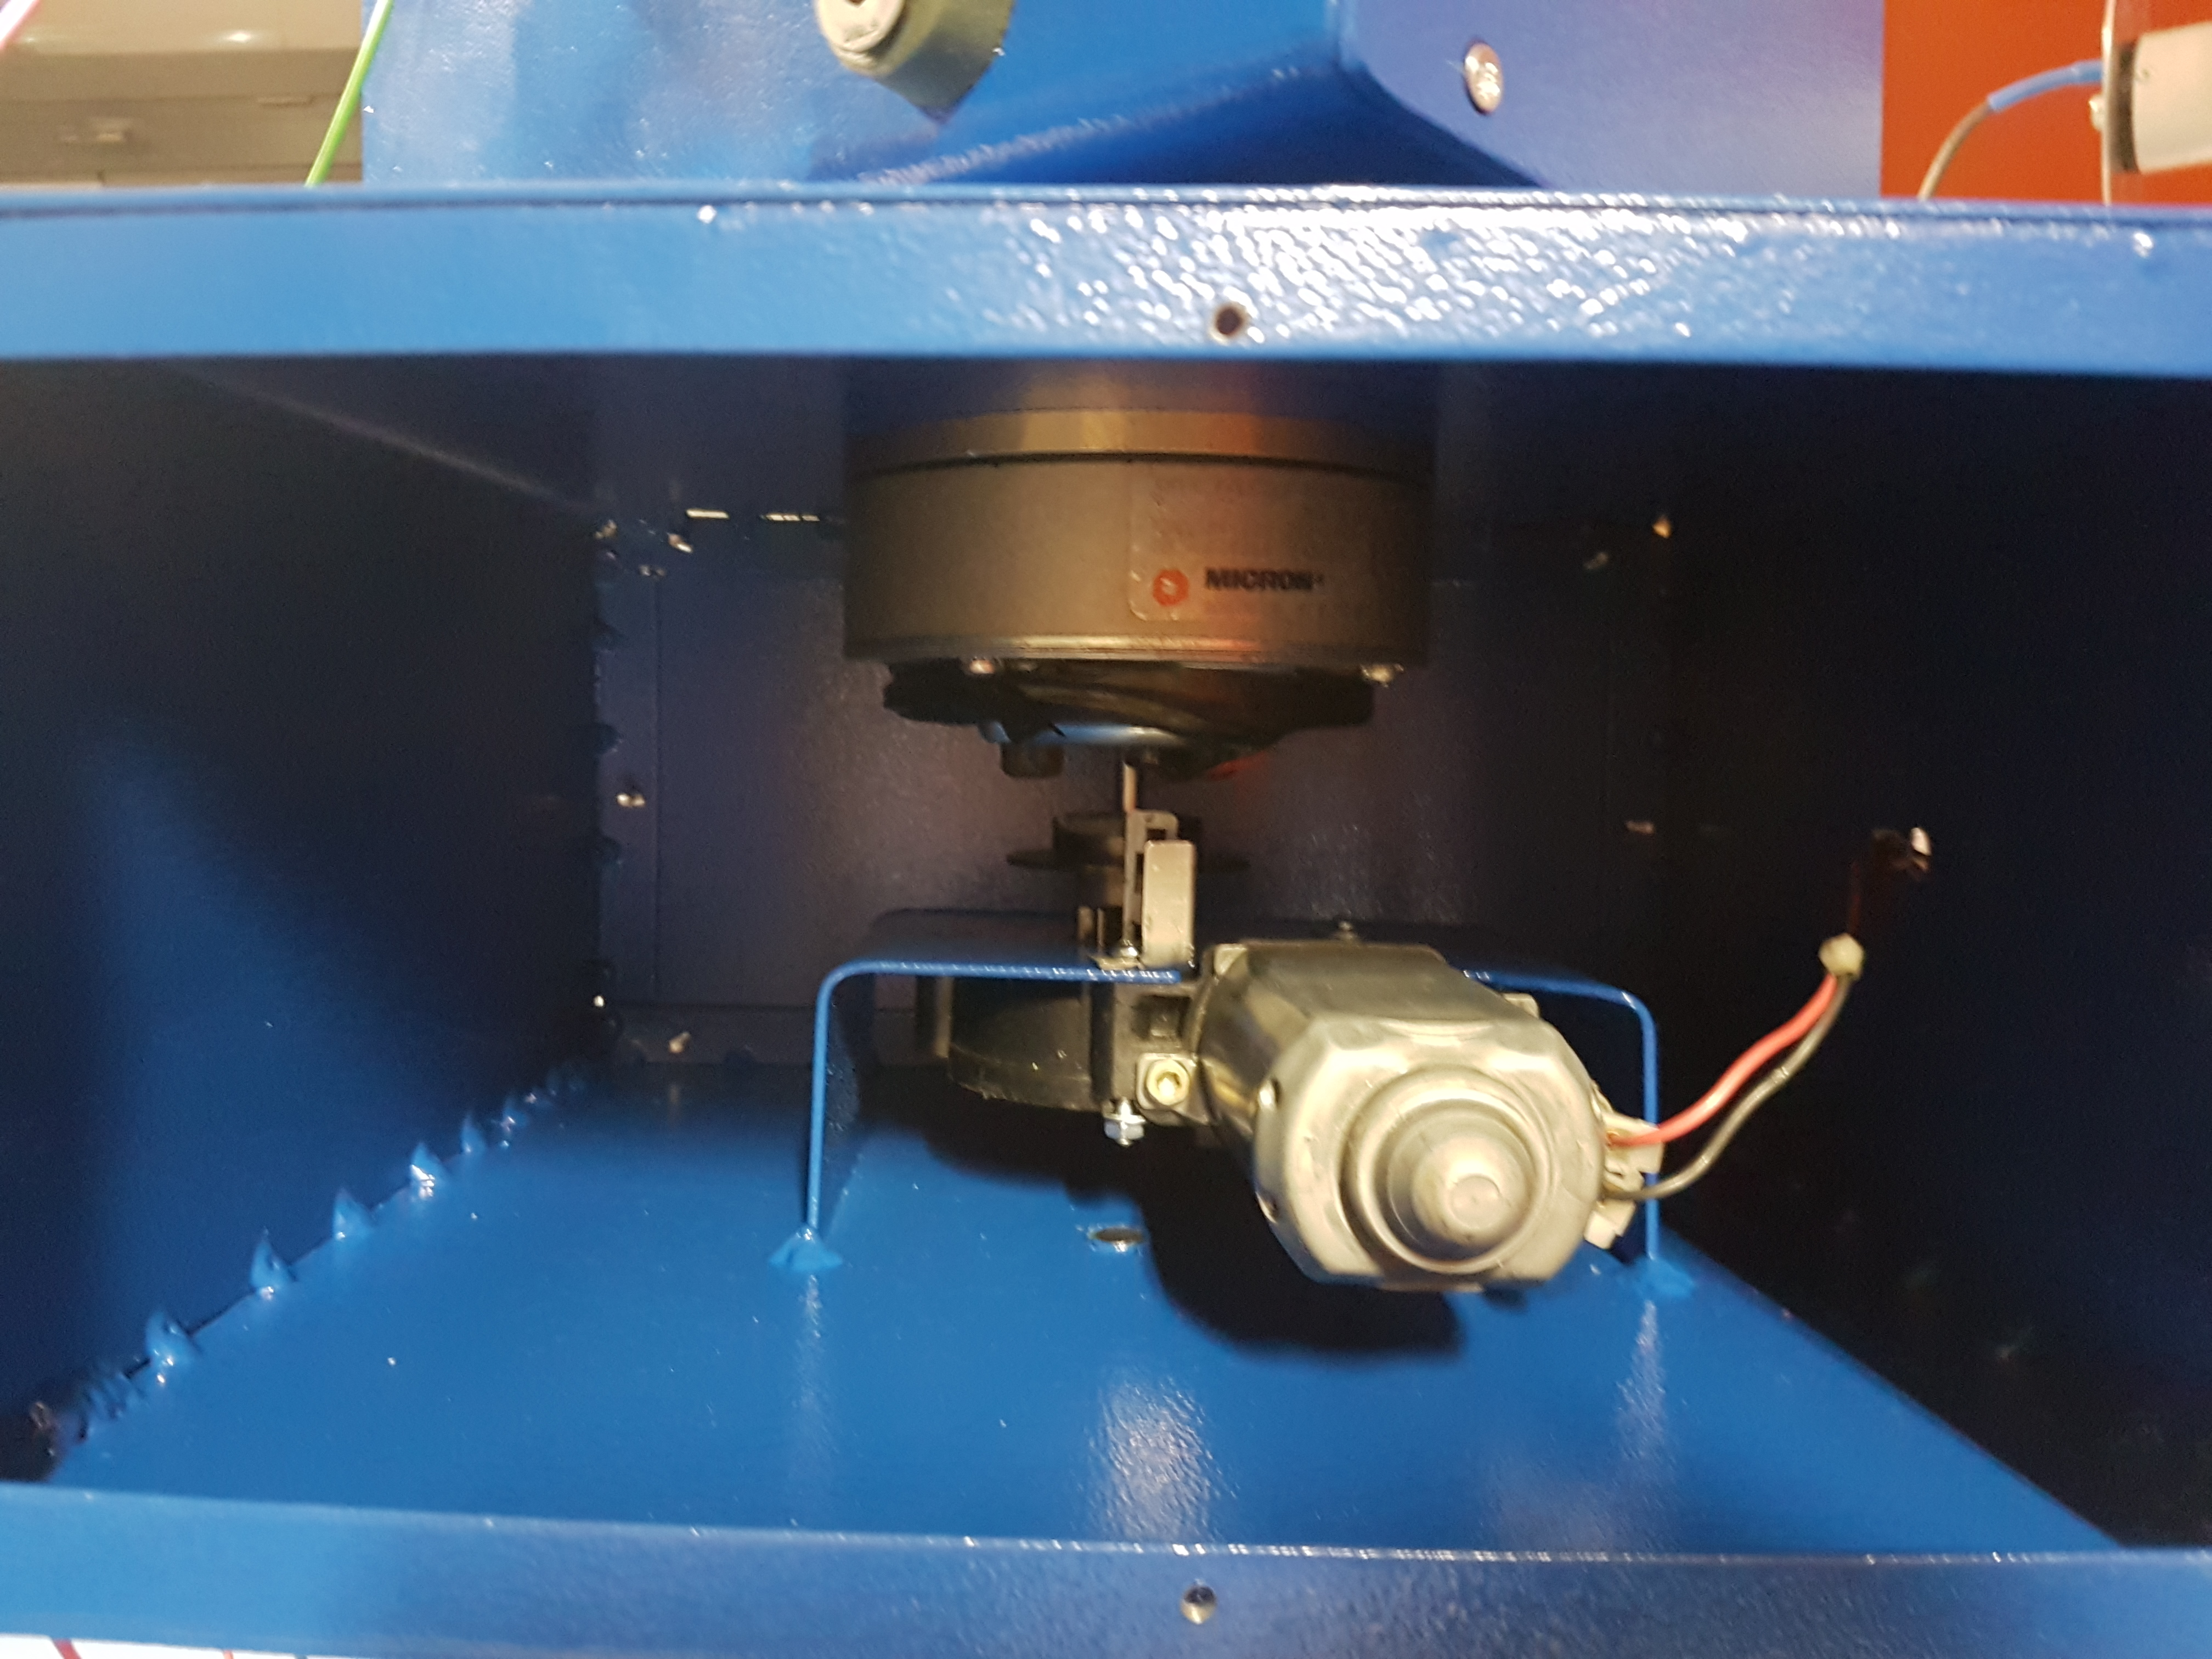
\includegraphics[width=0.7\textwidth]{rotor_dol}
 \centering
 \caption{Wnętrze dolnej części rotora}
 \label{rotdol}
\end{figure}

\begin{figure}[!htbp]
 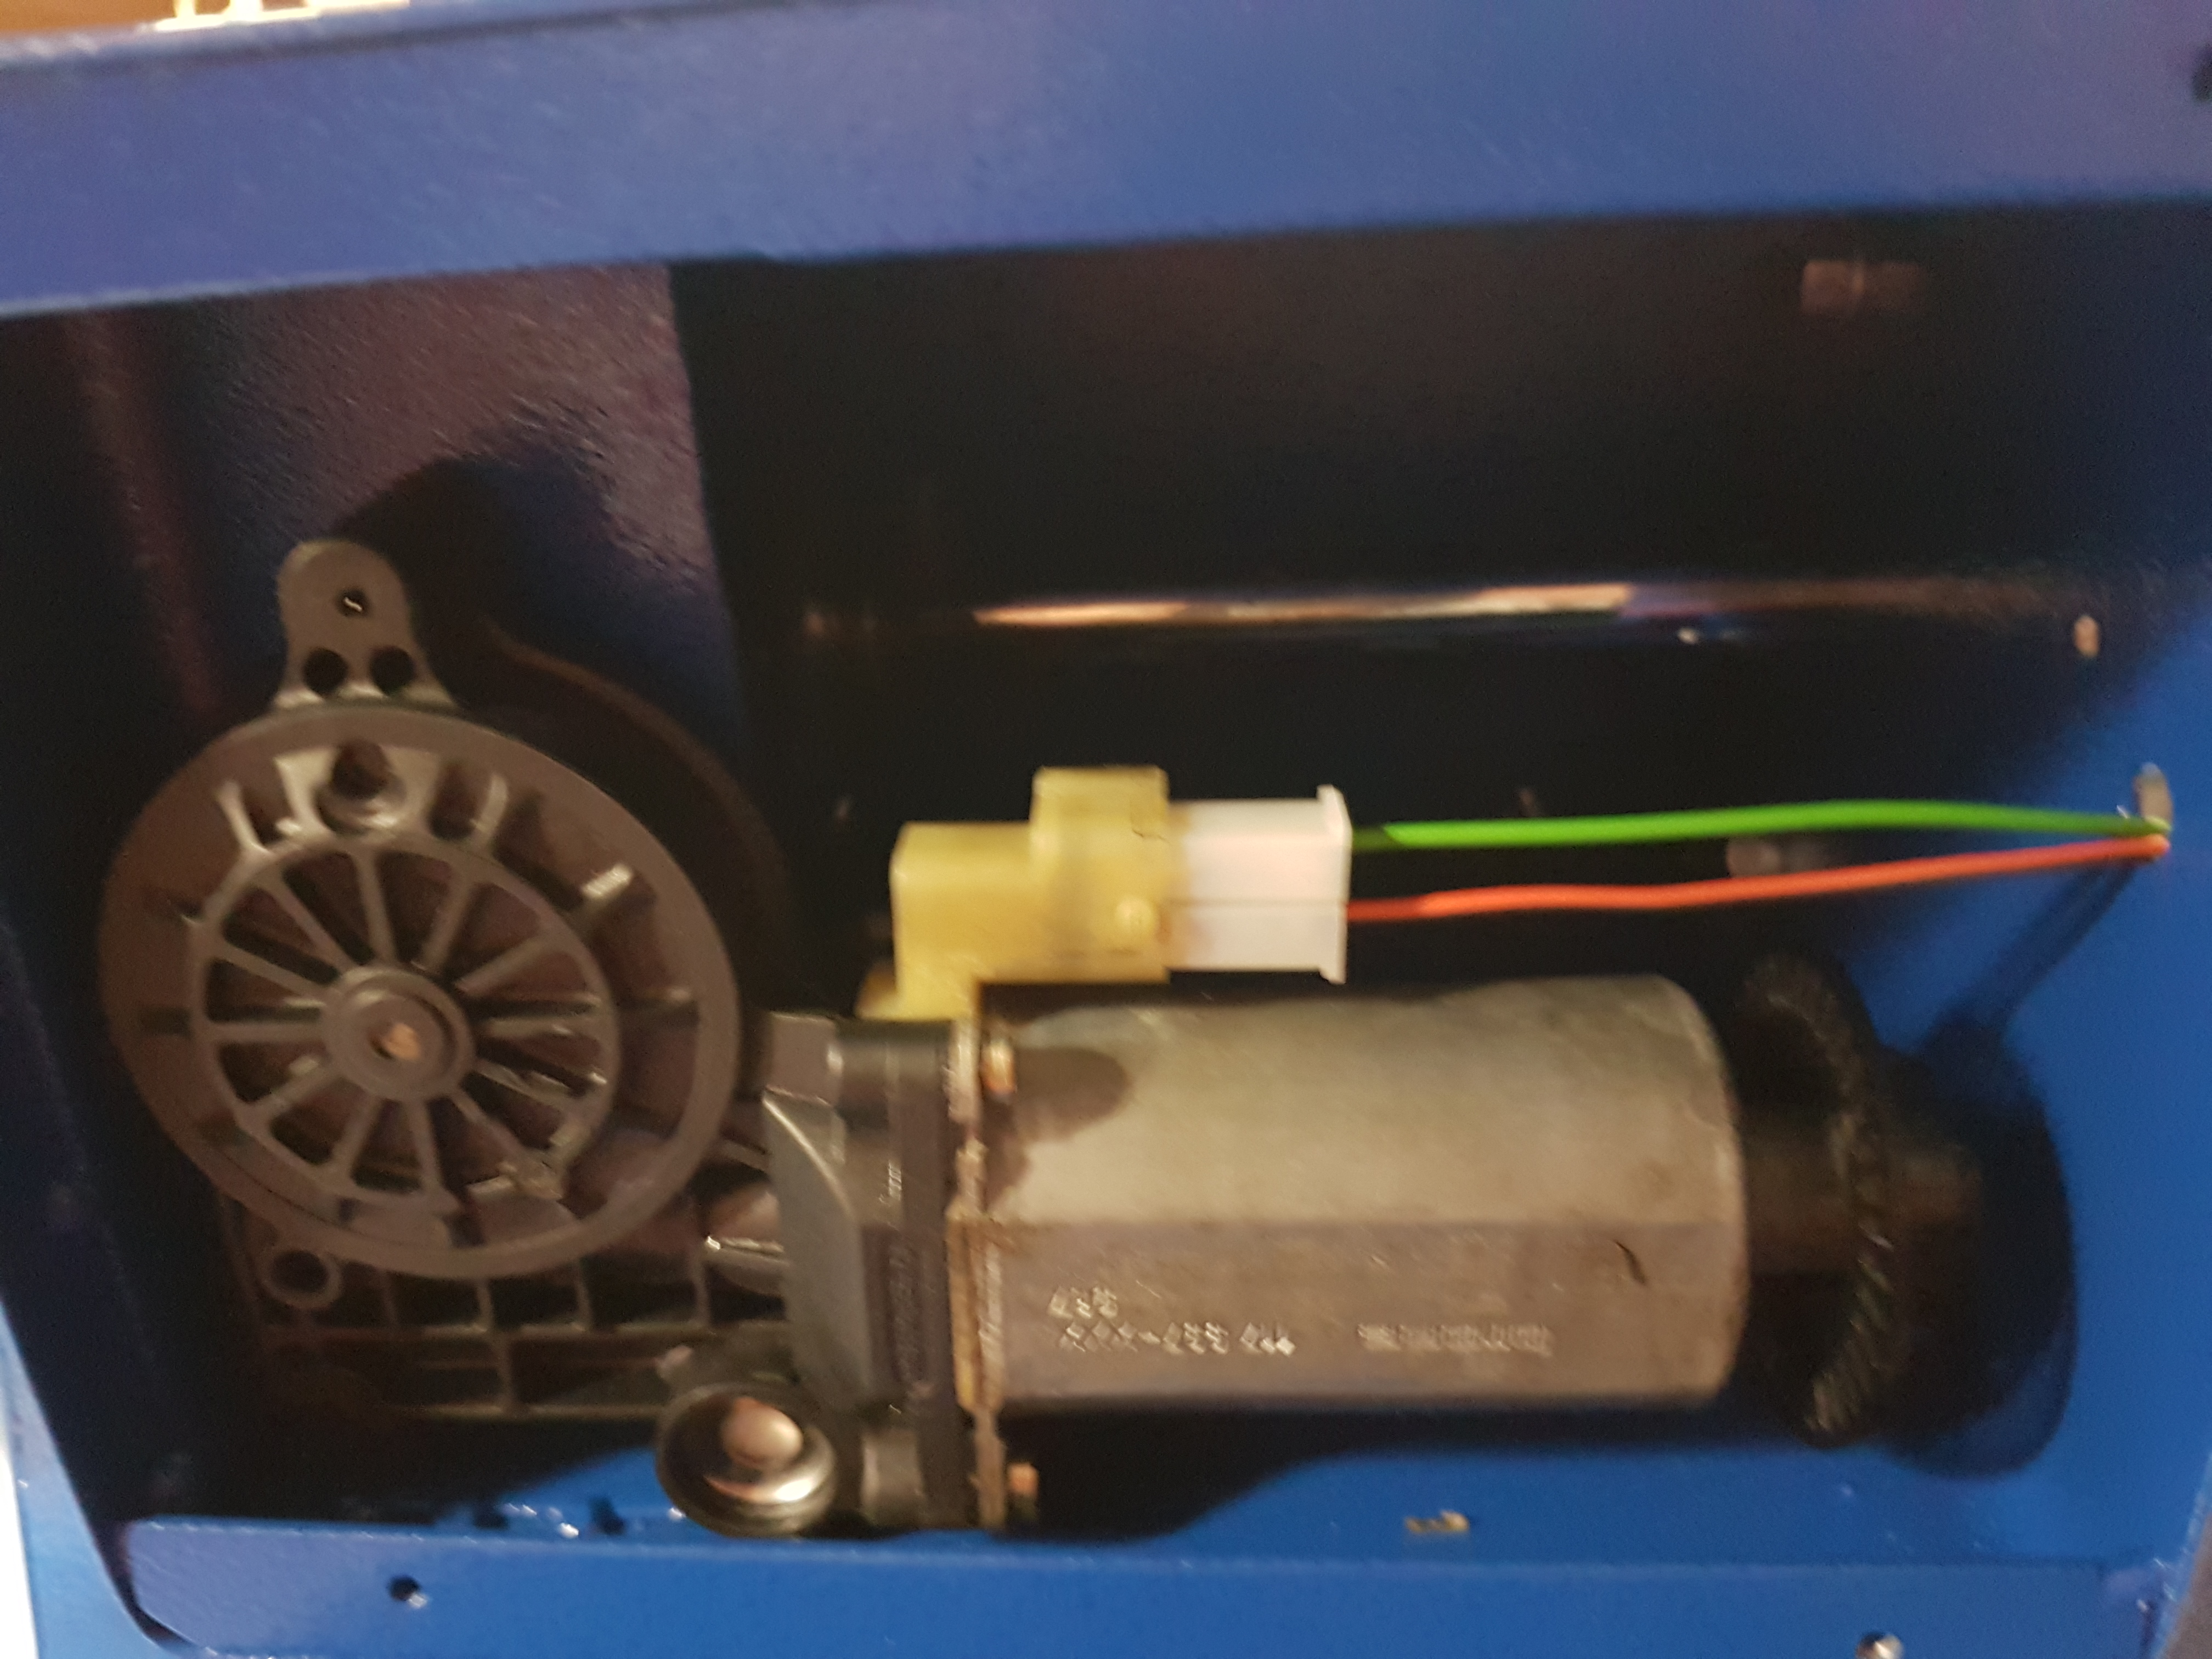
\includegraphics[width=0.7\textwidth]{rotor_gora}
 \centering
 \caption{Wnętrze górnej części rotora}
 \label{rotgora}
\end{figure}
